\documentclass[12pt]{article}

%Import packages
\usepackage{amsmath}
\usepackage{listings}
\usepackage[utf8]{inputenc}
\usepackage{algpseudocode}
\usepackage{algorithm}
\usepackage[]{hyperref}
\usepackage{url}
\usepackage{pgfgantt}
\usepackage{comment}
\usepackage{array}
\usepackage[section]{placeins}
\usepackage{array,xstring}
\usepackage{numprint} 
\usepackage{pdflscape} %%landscape
\usepackage{rotating}
\usepackage{graphicx}
\usepackage{csvsimple}
\usepackage{siunitx}

%%config indice, referencias, metadata.
\hypersetup{
    pdftitle={Tarea 2 PLN},
    bookmarksnumbered=true,     
    bookmarksopen=true,         
    bookmarksopenlevel=1,       
    colorlinks=true,            
    pdfstartview=Fit,           
    pdfpagemode=UseOutlines,
    pdfpagelayout=TwoPageRight,
    urlcolor=blue,
    linkcolor=blue,
    citecolor=red
}

% titulo
\title{Tarea 2 \\ IPLN \\ Grupo 9} 

% autores
\author{
  Valentina Da Silva 5.113.011-5\\
  Victor Díaz 4.295.936-0\\
  Leonardo Clavijo 5.054.830-5
}

\date{\today}


\begin{document}
\maketitle

\begin{abstract}
En este presente documento se procede a la explicación, tanto de la implementación de la aplicación, así como los parámetros de configuración necesarios para la ejecución de la misma.
\end{abstract}

\newpage
\tableofcontents
\newpage

\section{Introduction}
En la presente aplicación se trabajó en base a dos metodologías de procesamiento de datos, mediante el uso de WebServices y una aplicación local(LAN) del servicio Freeling mediante sockets.
Por lo tanto en la implementación contamos con dos modos de ejecución, esto puede ser útil para el caso de los usuarios que no cuenta con un servidor Freeling local, pero sí mediante una arquitectura orientada a servicios.
Al pensar en ambos casos, tenemos la ventaja de que si no contamos con alguno de ellos, podemos utilizar el otro método.

\section{Requerimientos}

\subsection{Librerías}\label{lib}
Para la correcta ejecución de la aplicación es necesario contar con el siguiente conjunto de librerías:
\begin{itemize}
  \item suds :  Para utilizar la aplicación mediante Webservices, se trata de una librería que permite la creación de estructuras orientadas a webservices, utilizando el protocolo SOAP.
  \item mathplotlib: Se utiliza para realizar las gráficas pertientes a los requerimientos del laboratorio.
  \item openpyxl : Librería utilizada para la lectura de archivos xls, para el caso en particular el archivo que contiene los comentarios a ser procesados.
\end{itemize}

Los mismas pueden ser agregadas fácilmente utilizando pip o easy-install.
\begin{itemize}
  \item suds : pip install suds-jurko | easy\_install suds-jurko.
  \item mathplotlib : pip install matplotlib | easy\_install -m matplotlib.
  \item openpyxl : pip install openpyxl | easy\_install openpyxl.
\end{itemize}


\subsection{Freeling}\label{free}
Para ejecutar la aplicación utilizando un servidor local, es necesario contar con la aplicación Freeling y ejecutarla en modo servidor, para ello se recurre a la siguiente orden vía línea de comandos:
$analyze$ $-f$ $./config/es.cfg$ $--flush$ $--server$ $--port$ $50005$ $\&$
Donde es.cfg es la configuración general de Freeling para lograr el correcto procesamiento del léxico en cuestión, de esto se tratará en la sección 'Configuraciones Freeling'\ref{configFree}; 50005 es el puerto en el que el servidor escucha los pedidos.
Una vez que se realizó este paso correctamente, podemos ejecutar nuestra aplicación Python. 

\subsubsection{Configuración}\label{configFree}
Los parámetros que se utilizaron para configurar Freeling en modo servidor fueron los siguientes(./config/es.cfg):
\begin{itemize}
\item AffixAnalysis=no : No es necesario en este caso.
\item MultiwordsDetection=yes : Se utiliza para detectar palabras múltiples en una 'string' ya que es habitual errores de tipeo como la falta de espacios o la introducción del caracter $.$ como separador.
\item NumbersDetection=yes : Opcional, se optó por introducirlo aunque aporte en menor proporción.
\item PunctuationDetection=yes : Detecta la puntuación que posteriormente se excluye de las palabras finales.
\item DatesDetection=no : No es necesario en este contexto, puesto que en esta categoría de comentarios no requiere tal precisión para procesar.
\item QuantitiesDetection=no : No es necesario procesar este tipo de magnitudes, se toma como una palabra cualquiera. 
\item DictionarySearch=yes : Para definir el lema, es útil que se encuentre en el diccionario para generar un tag correcto.
\item ProbabilityAssignment=yes : En algún caso podría ser necesario.
\item OrthographicCorrection=no : No sería una idea negativa utilizarlo, aunque para el caso no es una prioridad a tener en cuenta.
\item NERecognition=no : Identificar nombres por ejemplo no aporta calidad a la solución, además se observa comentarios como "Genial, Me Ha Atrapado la película", en realidad genera problemas cuando estamos agrupando las palabras positivas y negativas ya que con esta opción agruparía en un conjunto "Me Ha Atrapado" y se pedería lemas que aportan datos a la solución.
\end{itemize}
Estos fueron las configuraciones más importantes a tener en cuenta en el análisis morfológico, se deja a consideración el archivo ubicado en $./config/es.cfg$ para más detalles, además el mismo debe procesarse cuando se inicia el servicio de Freeling.


\section{Ejecución}
Para ejecutar la aplicación, únicamente se le debe brindar permisos de ejecución al archivo $tarea_1.py$, y mediante línea de comandos la siguiente orden:
$./tarea_1.py$
o $./tarea_1.py -w$ para ejecutarlo utilizando webservices anteriormente descripto.
\subsection{Parámetros}
Se brinda una serie de parámetros adicionales para la ejecución de la tarea.
\begin{itemize}
  \item -d: Muestra las gráficas en tiempo de ejecución, con la posibilidad de redimensionar las ventanas, entre otras propiedades interesantes a tener en cuenta.
  \item -v: Se utiliza para ejecutar la tarea en versión 1, es decir el programa se ejecuta utilizando la lista de palabras vacías de la primera entrega, no se genera filtro de lemas con el dominio del problema, los comentarios positivos corresponden a los valores 3,4 y 5.
  \item -w: Modo webservice, se ejecuta la aplicación realizando requests a un servicio web.
\end{itemize}

Una aclaración importante, la aplicación se ha probado exclusivamente en ambiente UNIX, desde la instalación de Freeling hasta las librerías de Python, ante funcionamientos anómalos en plataformas Windows, se sugiere que el programa sea ejecutado en UNIX.
Caso contrario de no disponer un entorno, igualmente puede ejecutarse el programa utilizando webservices. Aunque el funcionamiento no es óptimo los resultados son semejantes.

\section{Visualización}
Se muestra la interacción del sistema, según el modo de ejecución.

\begin{figure}[!h]
  \centering
    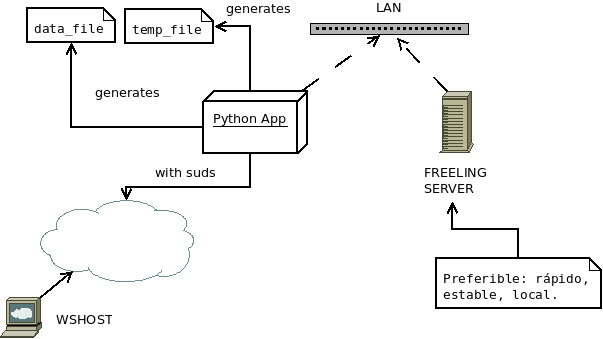
\includegraphics[width=0.8\textwidth]{./fig/arq.png}
  \caption{Interacción}
  \label{fig:arq}
\end{figure} 


\section{Implementación} \label{impl}
Se procede a la descripción de la implementación del programa. Para ello se utilizaron tres clases básicas para las configuraciones:
\begin{enumerate}
   \item Utils : que se encuentra en el mismo archivo a ejecutar $tarea_1.py$, la misma se encarga de realizar operaciones de lectura y escritura en los archivos, así como el porcesamiento de los datos utilizando Freeling.
   \item WebService : la misma se encuentra en el archivo webservices.py, se utiliza para cargar las especificaciones del servicio web en cuestión, además de brindar la implementación de solicitud y procesamiento de del léxico. Básicamente devuelve una lista con todas las palabras con su respectivo tag, lema y probabilidad.
   \item Classification : Esta clase es la responsable de todo lo relacionado con el clasificador de comentarios, utiliza el paquete nltk para generar un clasificador NaiveBayes.
 \end{enumerate} 

A continuación se describe las funciones definidas en el archivo $tarea_1.py$, específicamente de la clase utils.


\subsection{tarea\_1.py}
\subsubsection{loadXLSFile} \label{xlslib}
Encabezado: $def$ loadXLSFile(self). \\
Cuando se instancia la clase $Utils$, en sus atributos privados se encuentran ciertos parámetros que definen las condiciones a tener en cuenta para la lectura del archivo $.xlsx$, en particular el nombre del mismo $\_\_comment\_file$ y el rango de las celdas que deben ser procesadas($\_\_xls\_range$), básicamente utiliza la librería descrita en la sección anterior librería \ref{lib}, y devuelve como resultado el rango de celdas especificado por el parámetro en cuestión, el cual será iterado en la función main.


\subsubsection{loadStopwords}\label{func:loadSW}
Firma: $def$ loadStopwords(self, Ver=2). \\
En este caso se carga en un diccionario las palabras vacías que se suministran en el archivo $stopwords.txt$, se devuelve un diccionario para el rápido procesamiento posterior llevado a cabo. El parámetro $Ver$ con el valor en dos implica que se carga la lista de stopwords mejorada según el obligatorio 2, en caso contrario se procede a la carga con la lista brindada en la entrega anterior.


\subsubsection{loadSubjetiveElems}
Firma: $def$ loadSubjetiveElems(self). \\
Esta función carga el léxico proporcionado en el archivo $listaElementosSubjetivos.pl$, devolviendo un diccionario como estructura para su posterior procesamiento.

\subsubsection{loadDomain}\label{func:loadDomain}
Firma: $def$ loadDomain(self). \\
Básicamente abre el archivo $resources/dominio.txt$, y carga en un diccionario las palabras consideradas dentro del dominio del cine. En caso de que el archivo no se encuentre en el directorio especificado, se procede a lanzar una excepción correspondiente a dicho error.

\subsubsection{lematization\_freeling\_client}
Firma: $def$ lematization\_freeling\_client(self, comment). \\
Argumentos:
\begin{itemize}
  \item $comment$ : Comentario particular a ser procesado.
\end{itemize}
Su funcionalidad principal es tomar un comentario específico mediante una string, preprocesado anteriormente; se emplea sockets para la comunicación con el servidor Freeling, a diferencia de la primera entrega que utilizaba únicamente el servidor Freeling local y el uso de archivos auxiliares para procesar los pedidos. La ventaja de la utilización de sockets es que se puede ejecutar en ambientes remotos, desacomplando totalmente la aplicación del servidor. Básicamente devuelve una lista con lemas que cumplen ciertos criterios, como ser:
\begin{itemize}
  \item No se encuentra en la lista de palabras vacías.
  \item No se encuentra en la lista del dominio del problema.
\end{itemize}


\subsubsection{generateData}
Firma: $def$ generateData(self, allWords, filename). \\
Básicamente esta función se encarga de guardar en archivos con extensión $.csv$ las palabras procesadas durante la ejecución del programa. El parámetro allWords consiste en una lista de lemas que serán persistidos, mientras que $filename$ es el archivo destino. En la función principal del programa llamada $process$ se generan por medio de esta función los siguientes archivos:
\begin{itemize}
  \item negativeWords.csv : Contiene las palabras negativas encontradas en los comentarios.
  \item positiveWords.csv : Análogo al primero, aplicado a palabras positivas.
  \item allWords.csv : Se persisten todos los lemas involucrados en los comentarios. 
\end{itemize}


\subsubsection{generateStatisticData}
Firma: $def$ generateStatisticData(self, allWords, posWords, negWords, t, n). \\
Genera datos estadísticos para posterior análisis. Los parámetros $allWords$ consiste en una lista con todas las palabras, análogo para $posWords$ que son lemas positivos y $negWords$ lemas negativos, mientras que $t$ es la cantidad total de comentarios, $n$ la cantidad de comentarios negativos.
En la función principal $process$ se genera un archivo que contiene datos para formular conclusiones estadísticas, el mismo se encuentra en el directorio $res$ nombrado $Data.txt$ .


\subsubsection{plot} \label{func:plot}
Firma: $def$ plot(self, listaPlot, n\_groups, filename, totalwords). \\
Argumentos:
\begin{itemize}
  \item listaPlot : Contiene una lista ordenada con la siguiente tupla de datos $(Palabra, Comentarios)$, donde $Palabra$ es el lema a graficar, y $Comentario$ es la cantidad de veces comentarios en la que $Palabra$ está presente. Notar que se contabiliza únicamente una vez la palabra por comentario, para evitar casos extremos que degraden el comportamiento del programa en cuestión, ej. Comentario = "Hola, hola, hola, ...", si se evalúa globalmente, puede perjudicar el estudio en cuestión.
  \item n\_groups : Cantidad de palabras que serán procesadas en la salida gráfica.
  \item filename : Nombre del archivo de salida del procesamiento gráfico, la imagen será guardada en el directorio $figures$ localizado en la ruta donde se procesa la aplicación.
  \item totalwords : cantidad de lemas a ser procesados.
\end{itemize}

Su funcionalidad lo describe el nombre de la función, retorna una salida gráfica mediante archivos $.png$ con los resultados obtenidos.
En la implementación en cuestión se invoca cinco veces la presente función, generando los archivos a continuación:
\begin{itemize}
  \item AllWords.png : Se encuentran las $n\_groups$ palabras ordenadas de forma decreciente, en este caso no se distingue entre palabras positivas y negativas, básicamente es un conteo global de todas las palabras procesadas.
  \item NegativeSubjetive.png : En este caso se suministra el top $n\_groups$ palabras presentes en comentarios con un a puntuación 1 o 2 intersección palabras negativas suministradas en el archivo $listaElementosSubjetivos.pl$.
  \item PositiveSubjetive : Análogo al caso anterior pero aplicado a palabras positivas.
  \item NegativeWords.png : Ilustra las palabras presentes en los comentarios con evaluación negativa(1 y 2).
  \item PositiveWords.png : Análogo caso anterior pero teniendo en cuenta palabras con evaluación positiva.
\end{itemize}


\subsubsection{process}
Este bloque se encarga de tomar las funciones anteriormente mencionadas y procesar el algoritmo de forma adecuada.
Se presenta a continuación un pseudo-código de la implementación.



\begin{algorithmic}
  \State $xls \gets cargar\_comentarios()$
  \State $stopwords \gets cargar\_palabras\_vacias$
  \State $subjetivas \gets cargar\_palabras\_subjetivas$
  \State $domain \gets cargar\_dominio$
  
  \For{$comentario$ in $xls$}
    \State {$lista \gets lematizar(comentario)$}
     \For{$palabra$ in $lista$}
       \State {$(pos, neg) \gets agregarDiccionario()$}      
     \EndFor
  \EndFor
  
  \State $imagenes \gets graficarResultados(pos, neg)$
\end{algorithmic}
Las primeras cuatro líneas se compactan en la función de instanciación del objeto Utils, cargando entonces las palabras vacías, el dominio del problema, la lista de palabras subjetivas y los comentarios.
La simplicidad que brinda Python para el procesamiento de datos, básicamente resume el pseudocódigo en la implementación en sí misma, salvo detalles menores que requieren un procesamiento refinado.

\subsection{Classification.py}
Implementa la clase $Classificator$ encargada de clasificar los comentarios. A continuación se detallan las funciones que brinda dicha clase.

\subsubsection{loadComments}
Firma : $def$ loadComments(self). \\
Carga los comentarios en memoria a partir del archivo $.xlsx$ brindado, para realizar un procesamiento dinámico posteriormente, además de utilizar heurísticas que involucran el cuerpo del comentario y no el post procesamiento utilizando tokenización y análisis morfosintáctico.

\subsubsection{generate\_train\_set}
Firma : $def$ generate\_train\_set(self, large, prop, train\_name, test\_name). \\
Genera a través de la función $get\_train\_test\_set$ los índices de los comentarios que formarán parte del conjunto de comentarios de entrenamiento y test. A dichos índices los persiste en los archivos con nombre pasados por parámetro $train\_name$ y $test_name$ respectivamente. Los parámetros $large$ y $prop$ son la cantidad de comentarios en total y la proporción para el conjunto de entrenamiento(70 \%) respectivamente.

\subsubsection{get\_train\_test\_set}
Firma : $def$ get\_train\_test\_set(self, large, Prop). \\
Devuelve una lista con índices de los comentarios que serán incluídos en los conjuntos de entrenamiento y testing, se utilizan los parámetros $large$ y $Prop$ para determinar el tope de los comentarios y la proporción para el conjunto de entrenamiento. La lista que se genera se realiza de forma aleatoria, utilizando la clase $random$ que brinda python.

\subsubsection{generateHeuristic}
Firma: $def$ generateHeuristic(self, com). \\
Devuelve $True$ o $False$ en caso que el comentario $com$ posea un trigrama que forme parte de la heurística.


\subsubsection{feature}
Firma : $def$ feature(self, N, pcomment, comment, positive, negative, posSub, negSub). \\
Devuelve un diccionario con los atributos pertinentes al comentario $pcomment$, para generar los atributos se utiliza una lista de lemas generado anteriormente por la clase $Utils$ con la función $process$, consiste en la lista de lemas obtenida luego del análisis morfosintáctico. Para agregar atributos al comentario se tienen en cuenta tres tipos de atributos.
\begin{itemize}
  \item positive(lema) negative(lema) : Se generan a partir de los parámetros $positive$ y $negative$, que son diccionarios con los lemas positivos y negativos preprocesados, el atributo consiste básicamente si el comentario posee un lema de alguna de esos diccionarios, caso contrario también se agrega el atributo indicando que no lo posee. Por ejemplo el comentario $Bueno.$, supongamos que el lema "bueno" está incluído en el diccionario $positive$, por lo tanto dicho comentario obtendrá el atributo $positive(bueno) = True$.
  \item subjetive\_pos(lema) subjetive\_negative(lema) : El comentario se adjudicará esta clase de atributos si el mismo posee un lema que se encuentra en el diccionario de elementos subjetivos, tanto positivo como negativo. Supongamos que en el análisis morfosintáctico un lema del comentario es "malo", y dicho lema se encuentra en uno de los diccionarios $posSub$ o $negSub$, entonces el comentario será marcado con el atributo correspondiente $subjetive\_pos(lema)$ o $subjetive\_neg(lema)$ correspondiente a los diccionarios anteriores.
  \item $no\_gusto$ :  El comentario posee este atributo si se encuentra en $pcomentario$ alguna de las heurísticas planteadas, como por ejemplo "no me gusto", en caso de incluir una secuencia predeterminada que se define en $generateHeuristic$. Básicamente son trigramas que se estudiaron y se llegaron a la conclusión que aportan significancia estadística cuando se evalúan comentarios negativos.
\end{itemize}


\subsubsection{load\_train\_test\_set}
Firma: $def$ load\_train\_test\_set(self, train="./resources/train.txt", test="./resources/test.txt"). \\
Genera listas que contienen los índices de los comentarios incluídos en los conjuntos de entrenamiento y testing. Los parámetros $train$ y $test$ hacen referencia a la ruta de los archivos que contienen la información.

\subsubsection{saveMetrics}
Firma: $def$ saveMetrics(self, toSave, file\_name="./res/Metrics.txt"). \\
Dadas las métricas de calidad, como ser $accuracy$, $Precision$ y $Recall$ además de la matriz de confusión, son guardadas en el archivo $file\_name$. En la función principal $process$ de la presente clase, se persiste los datos automáticamente en el directorio $res$ con el nombre de archivo $Metrics.txt$.


\subsubsection{process}
Firma: $def$ process(self, posWords, negWords, posI, negI, tokenizedComm, train\_file="./resources/train.txt", test\_file="./resources/test.txt"). \\
Esta función se encarga básicamente de todo el procesamiento involucrando todas las funciones anteriormente mencionadas. Los pasos generados se detallan a continuación.
\begin{itemize}
  \item Se cargan en memoria los comentarios del archivo $.xlsx$.
  \item Se cargan en listas los conjuntos de entrenamiento y testing previamente generados.
  \item Con todos los comentarios que pertenecen al conjunto de entrenamiento, se generan los atributos y se almacenan en una lista que posteriormente será utilizada para instanciar el clasificador.
  \item Creación del clasificador, utilizando la lista mencionada en el paso anterior.
  \item Dado el conjunto de testing se clasifican los comentarios utilizando el clasificador, y se almacenan los resultados en diccionarios para el posterior análisis de métricas de calidad.
  \item Se generan métricas de calidad, la matriz de confusión y se imprimen los 20 atributos más utilizados.
\end{itemize}

Los parámetros $posWords$ y $negWords$ son diccionarios que contienen los lemas positivos y negativos procesados anteriormente por la clase $Utils$, $posI$ y $negI$ son la intersección de los lemas positivos y negativos con los elementos subjetivos. Mientras que $tokenizedComm$ es un diccionario con la lista de lemas para cada comentario procesado, se utiliza para evitar repetir la tarea de análisis morfosintáctico y aumentar el tiempo de respuesta del programa. Finalmente $train\_file$ y $test\_file$ contienen las direcciones de los archivos que contienen los índices de los comentarios que pertenecen al conjunto de entrenamiento y testeo.


\subsubsection{main}
Genera los 30 casos de prueba que se tendrán en cuenta para el análisis estadístico generado por el módulo $Statistics.py$.


\subsection{Statistics.py}

\subsubsection{doMetrics}
Firma: $def$ doMetrics(Display=False, WS=False, Ver=2). \\
Básicamente realiza el proceso de análisis morfosintáctico utilizando la clase $Utils$ y posteriormente clasifica los comentarios con los 30 conjuntos de entrenamiento y test, persisitiendo los datos obtenidos en el directorio $res/statistics$

\subsubsection{generateFile}
Firma: $def$ generateFile(metrics, outfile). \\
Dadas las métricas de calidad para los 30 casos de prueba $metrics$ se persisten las mismas en el archivo $outfile$, generando un archivo de salida $.csv$ que contienen las métricas $accuracy$, $precision$ y $recall$, además como los valores promedio para todos los casos.

\subsubsection{main}
Utiliza las dos funciones anteriormente mencionadas para generar las métricas de los 30 casos de prueba y persistirlos en los archivos $tabla1.csv$ y $tabla2.csv$. Archivos generados:
\begin{itemize}
  \item $tabla1.csv$: Contiene las métricas para los 30 casos de prueba procesados, se consideran los comentarios positivos con puntuación 4 y 5, y se utiliza el dominio y la lista mejorada de stopwords para un refinamiento de los lemas a procesar.
  \item $tabla2.csv$: Análogo al caso anterior pero los comentarios positivos poseen puntuación 3,4 y 5, no se utiliza dominio para filtrar lemas, ni la lista mejorada de stopwords. Básicamente se utiliza la versión 1 de la tarea para el procesamiento morfosintáctico.
\end{itemize}


\subsection{Eficiencia}
La complejidad del un programa se reduce a las estructuras utilizadas, la correcta utilización de las mismas implica un impacto directo sobre la eficiencia del programa. Para ello se utilizaron diccionarios para almacenar las palabras contenidas en los comentarios, de esta forma poder acceder en orden 1. La búsqueda se reduce a investigar si la llave(key) de indexado se encuentra presente en el diccionario. Por lo contrario, utilizando listas, la performance al procesar una lista mayor de comentarios tiene un impacto negativo en tiempos de ejecución.
Se recomienda fuertemente utilizar el modo de ejecución con servidor local con Freeling, de esta forma se reducen costos de tráfico de red y posibles "errores de ejecución" ajenas al programa diseñado.
La simplicidad de utilizar expresiones regulares para realizar reemplazos y búsquedas impacta positivamente en el desempeño del programa, es por ello que se utilizaron las mismas para sintetizar la lista de elementos subjetivos. Además agrega elegancia a la solución.
La captura de excepciones permite brindarle al usuario un detalle sobre los requerimientos que debe satisfacer para ejecutar correctamente el programa, para ello se implementó un manejo de las mismas en los casos de lectura y escritura de archivos así como también en el caso del WebService, que en ocasiones adversas no responde de forma adecuada.


\section{Análisis}
En las secciones anteriores se ha detallado aspectos de inicialización del ambiente para ejecutar la aplicación, así como las configuraciones pertinentes de Freeling, detalles sobre la implementación y algunas consideraciones sobre eficiencia. En este apartado se analizarán los resultados obtenidos luego de la ejecución del programa. Para ello en las siguientes subsecciones se detallarán los puntos requeridos en la letra del laboratorio.


\subsection{Información CORPUS}
Para esta consigna se utilizó la librería $openpyxl$ ya citada en la sección Librerías [\ref{lib}]. Básicamente se utilizó la función $loadXLSFile$ descrita en la sección Implementación [\ref{xlslib}], particularmente no se realizó un mapeo a memoria de los comentarios y sus respectivos puntajes, debido a que almacenar los mismos en estructuras internas como ser listas o diccionarios implica contar con memoria extra para ejecutar la aplicación. En lugar de ello se recorre el archivo $.xls$ brindado, haciendo lecturas del archivo en sí mismo, y no realizando el almacenamiento para su posterior lectura. Por lo tanto la información no se extrae completamente, pero sí parcialmente, con el fin de mejorar el rendimiento tanto en consumo de memoria como en la velocidad de ejecución del programa.
La lectura se realiza por medio de la función $loadXLSFile$ y posteriormente se recorre en la función $main$, 'lematizando' y realizando un análisis morfosintáctico, pero ello hace parte de la siguiente subsección.


\subsection{Procesamiento Información} \label{proc}
Como se mencionó anteriormente, las tareas de extracción de la información del CORPUS y el procesamiento de la información mediante Freeling se realizaron en paralelo con la finalidad de optimizar recursos y potenciar la eficiencia del programa. Para este punto se puede utilizar procesamiento mediante WebServices o un servidor Freeling local(recomendado), las configuraciones del servidor local se encuentran detalladas exhaustivamente en el archivo $es.cfg$ que se encuentra en el directorio $/config$. Los detalles particulares sobre la configuración de Freeling ya fueron mencionados[\ref{configFree}].
En la función $main$ se utiliza la función $lematizacion\_freeling\_client$ para procesar el comentario perteneciente al CORPUS, la cual tiene como retorno una lista de las palabras únicamente con el lema, puesto que el tag se utiliza para filtrar algunos elementos que no serán necesarios para el post procesamiento, en este caso se filtraron los siguientes tags:
\begin{itemize}
  \item $F$ : Denotan signos de puntuación, los cuales no consideraremos en nuestro análisis posterior.
  \item $Z$ : Los determinantes numerales tampoco son considerados en el análisis. 
\end{itemize}
Una vez que se cuenta con la lista de lemas de las palabras de un comentario, se almacenan en un diccionario usando como llave dicho lema, y como valor un dato del tipo Integer, con la finalidad de contabilizar la cantidad de veces que ocurre dicho lema en todos los comentarios a estudiar. Dicho conteo se realiza una vez por comentario, no la cantidad de ocurrencias global, con el fin de evitar comentarios con repetición de palabras que puedan interferir en el análisis de la muestra.
Se agregan los lemas en tres diccionarios, uno contiene todos los lemas procesados hasta el momento, y realiza el conteo global de todos los lemas independientemente del puntaje de un comentario. El segundo diccionario contiene únicamente los lemas que ocurren en comentarios evaluados con notas 1 y 2, mientras que el tercer diccionario almacena los lemas que ocurren en comentarios cuyo puntaje es 3,4 o 5. 


\subsection{Incorporar Recursos}
Este punto se realiza ejecutando las funciones descritas en la sección implementación[\ref{impl}], ellas son $loadSubjetiveElems$, la cual se encarga de incorporar el léxico suministrado en el archivo $listasElementosSubjetivos.pl$ y la función $loadStopwords$ que incorpora el archivo $stopwords.txt$ que contiene una lista con las palabras vacías, a modo de poder filtrar una cantidad mayor de palabras.
Ambos archivos se encuentran en el directorio $/resources$ junto con el .xls a procesar.
Las funciones retornan un diccionario con las palabras que se encuentran en los respectivos archivos, en el caso de los elementos subjetivos retorna dos diccionarios, uno con las palabras positivas y el otro las negativas, a modo de trabajar posteriormente con conjuntos y realizar las intersecciones pertinentes.

Se consideró oportuno mantener la información del obligatorio anterior, como son las secciones anteriores, ya que la tarea es incremental.

\subsection{Parte 1 :}
Para este requerimiento fue sencillo mejorar la lista de palabras vacías(stopwords), básicamente se generalizó la función \ref{func:loadSW} agregando un parámetro que indique si se debe cargar una lista en particular o la intersección de varias listas encontradas en la web.
En cuanto al requerimiento del dominio del problema, se generó una lista que se encuentra en un archivo llamado $dominio.txt$, ubicado en el directorio $/resources$. Para cargar esta lista de palabras, nuevamente se utilizó un diccionario para mejorar el proceso de búsqueda. Para más referencias observar la descripción de la función \ref{func:loadDomain}.
En el requerimiento que considera los comentarios positivos únicamente con la puntuación 4 y 5, se agregó el parámetro $Ver$, si el mismo posee el valor $2$, se excluyen los comentarios con puntuaciones 3, caso contrario se mantiene como en el obligatorio 1. Este argumento se agrega al instanciar la clase $Utils$, y depende del pasaje de parámetros cuando se ejecuta el programa, en caso de existir la opción $-v$, se considera la versión de la tarea 1, y por tanto los comentarios positivos contienen los valores 3,4 y 5. También vale la pena destacar que la presencia de este parámetro también condiciona los filtros sobre los lemas, utilizando listas de stopwords mejorada, así como el dominio del problema.

\subsection{Parte 2 :} \label{sub:part2}
Los atributos seleccionados fueron los siguientes:
\begin{itemize}
  \item $positive(string)$: Donde $string$ pertenece a los $N$ primeros lemas de la lista cuyos comentarios tuvieron una mención positiva, indicando si el lema está está presente o no en dicho comentario. Para ello se utiliza un atributo binario(True, False).
  \item $negative(string)$: Análogo al anterior, aplicado a los $N$ elementos de la lista con lemas donde los comentarios fueron evaluados con puntuación negativa.
  \item $subjetive\_pos(lema)$ : $lema$ pertenece a la lista de elementos subjetivos brindada, si en el comentario dicho lema pertenece, entonces se agrega el atributo mencionado.
  \item $subjetive\_neg(lema)$ : Análogo al anterior aplicado a la lista de elementos subjetivos negativos.
  \item $no\_gusto$ : Una heurística detectada es que en una gran proporción de comentarios negativos a procesar, poseen términos afectivos positivos, como ser 'gustó', sin embargo están contenidos en un contexto semejante a 'no me gustó' o semejante. Para ello se procedió a evaluar 2 palabras anteriores a los términos afectivos positivos, y en caso de encontrarse con una negación, se agrega el atributo mencionado. Nuevamente un atributo binario, demostrando la presencia o no de dicha heurística en el comentario.
\end{itemize}
Los atributos se analizaron con una selección aleatoria de comentarios, con la proporción requerida por la letra del obligatorio. Se realizaron pruebas con conjuntos distintos y se realizó un análisis estadístico de los datos, principalmente si el comportamiento del conjunto es normal, para ello se utilizaron test de normalidad de DAgostino y ejecutaron sobre 30 conjuntos distintos, ya que con dicho valor agrega un significado estadístico relevante. Si bien la letra del problema no requiere este procedimiento, se consideró oportuno observar si el conjunto seleccionado tiene impacto positivo o negativo en el momento de evaluar la calidad del clasificador. Para eso consideraremos la desviación estándar en los datos, así como la media de los valores $precision$ y $recall$, así como también $accuracy$. En el caso que los conjuntos seleccionados de forma aleatoria se comportan siguiendo una distribución normal, podemos establecer una cota en los atributos de calidad a evaluar, de esta forma también podemos asegurar que en promedio la calidad del clasificador es semejante, cualquiera sea el conjunto de datos tomado como referencia, con un márgen de error acotado.
Además para evaluar la calidad de las soluciones, no es suficiente tratar con un conjunto particular, puede ocurrir que al seleccionar un conjunto cualquiera, con la solución propuesta los atributos de calidad sean óptimos, pero no para un caso global. Entonces evaluar la solución sobre una cantidad significativa de conjuntos si brinda datos significativos sobre el comportamiento del clasificador de forma global y no particular.


\subsection{Parte 3 :}
Para esta sección utilizamos el coonjunto de libreríás $nltk$ para generar un clasificador. Para ello se creó una clase llamada $classification.py$ que cuenta con las funciones mencionadas en el apartado de la arquitectura del sistema. Básicamente las funciones principales a tratar en esta clase son las siguientes:
\begin{itemize}
  \item $generate\_train\_set$
  \item $feature$
\end{itemize}
La primera se utiliza para generar los conjuntos de entrenamiento y testing, utilizando una proporción $0.7$ para el conjunto de entrenamiento.
La segunda función agrega los atributos a los comentarios en cuestión, descriptos en la sección anterior[\ref{sub:part2}].
Como se mencionó anteriormente se evaluó el comportamiento a partir de 30 conjuntos de entrenamientos distintos, tanto para los comentarios positivos con puntuación 3,4 y 5 así como los que excluyen el puntaje 3 del conjunto.
Los resultados obtenidos en esta parte se presentan en la sección Estadístico[\ref{sub:estad}], con dichos valores se procederá a tomar conclusiones adecuadas a la calidad del clasificador generado, dependiendo también de qué se considera como comentario positivo.
La generación del conjunto de entrenamiento se realizó de forma aleatoria, para evitar linealidad en la selección de los comentarios, influyendo de forma negativa en el momento de evaluar la calidad del clasificador. Para ello se toma la cantidad de comentarios en el Corpus y se toma aleatoriamente $0.7$ de los mismos, los restantes formarán parte del conjunto de testing. Cabe mencionar que por facilidad en la ejecución del programa, se guarda en un archivo $test.txt$ y $train.txt$ los números relativos a los comentarios seleccionados.

\npdecimalsign{.}
\nprounddigits{3}

\subsection{Estadístico} \label{sub:estad}
Para la obtención de los resultados, se implementó el módulo $Statistics.py$, el mismo utiliza los módulos $tarea_1.py$ y $classification.py$, toma los 30 conjuntos de entrenamiento anteriormente generados y clasifica los comentarios según los mismos. Además posee la funcionalidad de generar las tablas presentes en esta sección.
Se obtuvieron los siguientes resultados[\ref{tabla:1}] generando 30 conjuntos aleatorios de entrenamiento y test, los resultados obtenidos implican que el $accuracy$ del clasificador es de aproximadamente 80\%, el mejor caso se obtuvo en el conjunto de número 25, donde el $accuracy$ se aproximó a un 84 \%. Este estudio demuestra en un caso global, ya que con una cantidad apreciable de conjuntos distintos podemos obtener significancia estadística en el momento de evaluar el clasificador en forma genérica.
En la tabla \ref{tabla:2} tenemos los resultados incluyendo las puntuaciones 3 como comentarios positivos. Intuitivamente se podría decir que eliminando los comentarios con puntuación 3 tanto para entrenar el clasificador, como para evaluar los comentarios con ese puntaje, se obtendrían mejores resultados, pero en cambio las tablas demuestran esa hipótesis. Analizando la segunda tabla, podemos decir que los comentarios con puntuación 3 tiene un impacto impacto nulo cuando se clasifican los comentarios positivos, sin embargo en el momento de evaluar los negativos el desempeño es inferior al clasificador entrenado con un conjunto de comentarios excluyendo puntuaciones 3. Esto es un dato interesante para considerar, si tomamos el caso número $25$ tenemos un $accuracy$ de $84.7 \%$ apenas superior al de la primera tabla. Cuando contrastamos con las métricas $Recall$ y $Precision$ concluímos que para el caso 1, existe una leve mejora respecto al caso 2.
Algunos detalles del estudio estadístico como ser la desviación estándar, y el test de normalidad de D Agostino se brindan en la tabla \ref{tabla:datos}. Para éste último como utilizamos un tamaño de muestra de 30 conjuntos, evaluaremos con un $\alpha = 0.02$ y a partir de esto tenemos las siguientes cotas  $[0.2622 , 0.2871]$, en el caso que el resultado del test de normalidad sea un valor que pertenece a dicho conjunto, la muestra es normal, por lo cual podemos utilizar como referencia para el planteo de conclusiones en cuanto a la calidad del clasificador se refiere.
Los casos propuestos se resumen:
\begin{itemize}
  \item Caso 1: Evaluación excluyendo comentarios con puntuación igual a 3.
  \item Caso 2: Evaluación incluye comentarios con puntuación igual a 3, dentro de la categoría positivos.
\end{itemize}
Se tomó como referencia todos los atributos de calidad planteados, la nomenclatura se detalla en el siguiente numerado:
\begin{itemize}
  \item ACC: Accuracy.
  \item PP: Precision Positive, métrica Precision aplicada a los comentarios positivos.
  \item RP: Recall Positive, métrica Recall aplicada a los comentarios positivos.
  \item PN: Precision Negative, métrica Precision aplicada a los comentarios negativos.
  \item RN: Recall Negative, métrica Recall aplicada a los comentarios negativos.
\end{itemize}

Las conclusiones que se pueden observar a partir de la tabla es que se puede tomar cualquier métrica como referencia, puesto que al realizar el test de normalidad efectivamente estamos comprobamos que para los datos, se comportan siguiendo una distribución normal.
A partir de estos datos podemos comparar los dos casos propuestos de forma independiente según la métrica deseada, tomando la media como referencia y estableciendo qué atributo es mejor para los dos casos planteados.
Podemos decir entonces que para el Caso 1, se obtiene una mejor evaluación de los comentarios negativos, mientras que para los positivos en ambos casos las métricas son semejantes. Por tanto a nivel global con la métrica $accuracy$ el clasificador con distintos dominios de comentarios se comporta de forma similar, teniendo ventaja el primer clasificador excluyendo los comentarios con puntuaciones 3 de la clasificación positiva.
\begin{table}
\begin{center}
    \begin{tabular}{| c | c | c | c | c |}
    \cline{2-5}
    \multicolumn{1}{c}{}&
    \multicolumn{2}{|c}{Caso 1}&
    \multicolumn{2}{|c|}{Caso 2} \\ \hline
    
    \multicolumn{1}{|c}{Métrica}&
    \multicolumn{1}{|c}{$\sigma$}&
    \multicolumn{1}{|c}{$DA$}&
    \multicolumn{1}{|c}{$\sigma$}&
    \multicolumn{1}{|c|}{$DA$} \\ \hline
    ACC & 0.026003 & 0.28689 & 0.016380 & 0.27771 \\ \hline
    PP & 0.027385 & 0.28140 & 0.021212 & 0.27720 \\ \hline
    RP & 0.024598 & 0.27735 & 0.017131 & 0.28631 \\ \hline
    PN & 0.074322 & 0.27949 & 0.052173 & 0.27693 \\ \hline
    RN & 0.065168 & 0.27797 & 0.054888 & 0.27498 \\ \hline
    \end{tabular}
\end{center}
    \caption{Datos Estadísticos}
    \label{tabla:datos}
\end{table}



\begin{table}[!htb]
\begin{center}
\begin{tabular}{|l |N{1}{3} | N{1}{3} | N{1}{3} | N{1}{3} | N{1}{3} |} 
\hline
 \multicolumn{1}{|l}{Caso}&
 \multicolumn{1}{|l}{Accuracy}&
 \multicolumn{1}{|l}{PP}&
 \multicolumn{1}{|l}{RP}&
 \multicolumn{1}{|l}{PN}&
 \multicolumn{1}{|l|}{RN}
\tabularnewline
  \hline
  1 & 0.7727272727272727 & 0.8395061728395061 & 0.85 & 0.5862068965517241 & 0.5666666666666667 \tabularnewline
2 & 0.8340807174887892 & 0.8604651162790697 & 0.9192546583850931 & 0.7450980392156863 & 0.6129032258064516 \tabularnewline
3 & 0.7545454545454545 & 0.7758620689655172 & 0.9 & 0.6739130434782609 & 0.44285714285714284 \tabularnewline
4 & 0.7743362831858407 & 0.8214285714285714 & 0.8679245283018868 & 0.6379310344827587 & 0.5522388059701493 \tabularnewline
5 & 0.7909090909090909 & 0.8363636363636363 & 0.8789808917197452 & 0.6545454545454545 & 0.5714285714285714 \tabularnewline
6 & 0.7899543378995434 & 0.8372093023255814 & 0.8888888888888888 & 0.6170212765957447 & 0.5087719298245614 \tabularnewline
7 & 0.8051948051948052 & 0.8786127167630058 & 0.8636363636363636 & 0.5862068965517241 & 0.6181818181818182 \tabularnewline
8 & 0.8251121076233184 & 0.8538011695906432 & 0.9125 & 0.7307692307692307 & 0.6031746031746031 \tabularnewline
9 & 0.8362068965517241 & 0.888268156424581 & 0.8983050847457628 & 0.660377358490566 & 0.6363636363636364 \tabularnewline
10 & 0.8311111111111111 & 0.8342541436464088 & 0.949685534591195 & 0.8181818181818182 & 0.5454545454545454 \tabularnewline
11 & 0.8165137614678899 & 0.8392857142857143 & 0.9155844155844156 & 0.74 & 0.578125 \tabularnewline
12 & 0.832579185520362 & 0.8802395209580839 & 0.8963414634146342 & 0.6851851851851852 & 0.6491228070175439 \tabularnewline
13 & 0.7623318385650224 & 0.8109756097560976 & 0.8580645161290322 & 0.6271186440677966 & 0.5441176470588235 \tabularnewline
14 & 0.8165137614678899 & 0.8360655737704918 & 0.9386503067484663 & 0.7142857142857143 & 0.45454545454545453 \tabularnewline
15 & 0.8283261802575107 & 0.8674033149171271 & 0.9075144508670521 & 0.6923076923076923 & 0.6 \tabularnewline
16 & 0.8270042194092827 & 0.8638743455497382 & 0.9166666666666666 & 0.6739130434782609 & 0.543859649122807 \tabularnewline
17 & 0.7897196261682243 & 0.8404907975460123 & 0.8782051282051282 & 0.6274509803921569 & 0.5517241379310345 \tabularnewline
18 & 0.8464912280701754 & 0.8655913978494624 & 0.9415204678362573 & 0.7619047619047619 & 0.5614035087719298 \tabularnewline
19 & 0.8296943231441049 & 0.8659217877094972 & 0.9117647058823529 & 0.7 & 0.5932203389830508 \tabularnewline
20 & 0.8348623853211009 & 0.8606060606060606 & 0.9161290322580645 & 0.7547169811320755 & 0.6349206349206349 \tabularnewline
21 & 0.8651162790697674 & 0.88 & 0.9506172839506173 & 0.8 & 0.6037735849056604 \tabularnewline
22 & 0.7894736842105263 & 0.8545454545454545 & 0.8545454545454545 & 0.6190476190476191 & 0.6190476190476191 \tabularnewline
23 & 0.8532110091743119 & 0.8820224719101124 & 0.9345238095238095 & 0.725 & 0.58 \tabularnewline
24 & 0.8230088495575221 & 0.8488372093023255 & 0.9125 & 0.7407407407407407 & 0.6060606060606061 \tabularnewline
25 & 0.8122270742358079 & 0.8681318681318682 & 0.8926553672316384 & 0.5957446808510638 & 0.5384615384615384 \tabularnewline
26 & 0.8088888888888889 & 0.8222222222222222 & 0.9308176100628931 & 0.7555555555555555 & 0.5151515151515151 \tabularnewline
27 & 0.8258928571428571 & 0.8662790697674418 & 0.9030303030303031 & 0.6923076923076923 & 0.6101694915254238 \tabularnewline
28 & 0.8063063063063063 & 0.8547486033519553 & 0.9 & 0.6046511627906976 & 0.5 \tabularnewline
29 & 0.7385321100917431 & 0.8 & 0.8366013071895425 & 0.5689655172413793 & 0.5076923076923077 \tabularnewline
30 & 0.762114537444934 & 0.8452380952380952 & 0.8352941176470589 & 0.5254237288135594 & 0.543859649122807 \tabularnewline
AVG & 0.8094328727583726 & 0.8492750057348091 & 0.8986734119014108 & 0.6771523582988307 & 0.5664432145348967 \tabularnewline

  \hline
\end{tabular} 
\end{center}
\caption{Métricas conjuntos} 
\label{tabla:1}
\end{table}

\begin{table}[!htb]
\begin{center}
\begin{tabular}{|l |N{1}{3} | N{1}{3} | N{1}{3} | N{1}{3} | N{1}{3} |} 
\hline
 \multicolumn{1}{|l}{Caso}&
 \multicolumn{1}{|l}{Accuracy}&
 \multicolumn{1}{|l}{PP}&
 \multicolumn{1}{|l}{RP}&
 \multicolumn{1}{|l}{PN}&
 \multicolumn{1}{|l|}{RN}
\tabularnewline
  \hline
  1 & 0.7709923664122137 & 0.8736842105263158 & 0.8217821782178217 & 0.5 & 0.6  \tabularnewline
2 & 0.7938931297709924 & 0.8724489795918368 & 0.855 & 0.5606060606060606 & 0.5967741935483871 \tabularnewline
3 & 0.7633587786259542 & 0.8037383177570093 & 0.8958333333333334 & 0.5833333333333334 & 0.4 \tabularnewline
4 & 0.7748091603053435 & 0.8207547169811321 & 0.8923076923076924 & 0.58 & 0.43283582089552236 \tabularnewline
5 & 0.7709923664122137 & 0.8492462311557789 & 0.8492462311557789 & 0.5238095238095238 & 0.5238095238095238 \tabularnewline
6 & 0.7938931297709924 & 0.8544600938967136 & 0.8878048780487805 & 0.5306122448979592 & 0.45614035087719296 \tabularnewline
7 & 0.816793893129771 & 0.8767772511848341 & 0.893719806763285 & 0.5686274509803921 & 0.5272727272727272 \tabularnewline
8 & 0.8396946564885496 & 0.8829268292682927 & 0.9095477386934674 & 0.6842105263157895 & 0.6190476190476191 \tabularnewline
9 & 0.8129770992366412 & 0.8726415094339622 & 0.893719806763285 & 0.56 & 0.509090909090909 \tabularnewline
10 & 0.8473282442748091 & 0.8644859813084113 & 0.9438775510204082 & 0.7708333333333334 & 0.5606060606060606 \tabularnewline
11 & 0.8091603053435115 & 0.8663366336633663 & 0.8838383838383839 & 0.6166666666666667 & 0.578125 \tabularnewline
12 & 0.8129770992366412 & 0.8714285714285714 & 0.8926829268292683 & 0.5769230769230769 & 0.5263157894736842 \tabularnewline
13 & 0.7900763358778626 & 0.8293838862559242 & 0.9020618556701031 & 0.6274509803921569 & 0.47058823529411764 \tabularnewline
14 & 0.8129770992366412 & 0.8691588785046729 & 0.8985507246376812 & 0.5625 & 0.4909090909090909 \tabularnewline
15 & 0.7709923664122137 & 0.8585858585858586 & 0.8415841584158416 & 0.5 & 0.5333333333333333 \tabularnewline
16 & 0.8396946564885496 & 0.8687782805429864 & 0.9365853658536586 & 0.6829268292682927 & 0.49122807017543857 \tabularnewline
17 & 0.767175572519084 & 0.8666666666666667 & 0.8284313725490197 & 0.47761194029850745 & 0.5517241379310345 \tabularnewline
18 & 0.8778625954198473 & 0.9219512195121952 & 0.9219512195121952 & 0.7192982456140351 & 0.7192982456140351 \tabularnewline
19 & 0.8244274809160306 & 0.8792270531400966 & 0.896551724137931 & 0.6181818181818182 & 0.576271186440678 \tabularnewline
20 & 0.8015267175572519 & 0.8585365853658536 & 0.8844221105527639 & 0.5964912280701754 & 0.5396825396825397 \tabularnewline
21 & 0.8053435114503816 & 0.895 & 0.8564593301435407 & 0.5161290322580645 & 0.6037735849056604 \tabularnewline
22 & 0.7938931297709924 & 0.8606965174129353 & 0.8693467336683417 & 0.5737704918032787 & 0.5555555555555556 \tabularnewline
23 & 0.8282442748091603 & 0.8957345971563981 & 0.8915094339622641 & 0.5490196078431373 & 0.56 \tabularnewline
24 & 0.7938931297709924 & 0.865979381443299 & 0.8571428571428571 & 0.5882352941176471 & 0.6060606060606061 \tabularnewline
25 & 0.8015267175572519 & 0.8761904761904762 & 0.8761904761904762 & 0.5 & 0.5 \tabularnewline
26 & 0.8015267175572519 & 0.8333333333333334 & 0.9183673469387755 & 0.6521739130434783 & 0.45454545454545453 \tabularnewline
27 & 0.8244274809160306 & 0.8944723618090452 & 0.8768472906403941 & 0.6031746031746031 & 0.6440677966101694 \tabularnewline
28 & 0.8053435114503816 & 0.8697674418604651 & 0.8904761904761904 & 0.5106382978723404 & 0.46153846153846156 \tabularnewline
29 & 0.7519083969465649 & 0.851063829787234 & 0.8121827411167513 & 0.5 & 0.5692307692307692 \tabularnewline
30 & 0.7824427480916031 & 0.8627450980392157 & 0.8585365853658536 & 0.5 & 0.5087719298245614 \tabularnewline
AVG & 0.802671755725191 & 0.8655400263934292 & 0.8812186014648714 & 0.5777741499601223 & 0.5388865664091044 \tabularnewline

  \hline
\end{tabular} 
\end{center}
\caption{Métricas conjuntos} 
\label{tabla:2}
\end{table}


\subsection{Parte 4}
Para esta subsección posteriormente a un análisis estadístico que involucra varios conjuntos de estudio, se selecciona un conjunto independiente a los del caso de prueba, si bien las métricas obtenidas están acotadas por lo cual se centrará particularmente en la generación de la matriz de confusión, así como las métricas $Precision$ y $Recall$.

Se establece la separación de conjuntos en comentarios negativos y positivos, evaluado $Recall$ y $Precision$.
\begin{itemize}
  \item Accuracy: 0.8078
  \item Precision Positive: 0.8474
  \item Recall Positive: 0.8982
  \item Precision Negative: 0.6730
  \item Recall Negative: 0.5645
\end{itemize}

La matriz de confusión pertinente queda representada en la tabla \ref{tabla:matrix}, los valores en la diagonal indican los casos Verdadero-Positivo, mientras que cualquier otra celda que no corresponde a la diagonal indica que la clasificación del comentario es errónea. Como podemos observar, la correcta clasificación de los comentarios existe en mayor proporción cuando los comentarios poseen una valoración positiva. La proporción de comentarios negativos correctamente clasificados apenas supera el $50 \%$, lo cual implica que el rendimiento del clasificador es estrechamente superior en el momento de evaluar comentarios positivos.
$Precision$ es una métrica que se evalúa según la siguiente ecuación:
\begin{equation}
  Precision = \frac{TP}{TP + FP}
\end{equation}
Entonces esta métrica nos reporta el porcentaje de acierto en la clasificación, observar que $Precision$ se maximiza cuando $FP=0$, es decir que no existen Falsos-Positivos es decir, el clasificador evaluó correctamente todos los comentarios.
En cambio tenemos la ecuación de $Recall$:
\begin{equation}
  Recall = \frac{TP}{TP + FN}
\end{equation} 
Análogo al anterior pero define la métrica en proporción a los Falsos-Negativos obtenidos por el clasificador.
Con los datos obtenidos, podemos decir que el clasificador no posee un comportamiento óptimo, si evaluamos el clasificador en un CORPUS distinto, pero aplicado al mismo dominio del cine donde predominen comentarios negativos, posiblemente el clasificador sea correctamente entrenado, mejorando los resultados en gran proporción.
Vale la pena destacar que existe anomalía en ciertos comentarios, como no corresponder la puntuación con el cuerpo del comentario, un ejemplo claro es la contradicción de cierto usuario cuyo comentarios es "Muy bueno!", y el puntaje asignado corresponde a un 2. Estas anomalías no están al alcance del clasificador si no se tiene un dominio suficientemente extenso como para llegar a la conclusión que el lema "bueno", condiciona que el comentario sea negativo. En otras palabras, es más probable que dicho lema corresponda a un comentario cuya puntuación sea positiva. Sin embargo, existen comentarios de la forma "No me gusta", en los cuales si bien contiene un lema que pondera a comentarios positivos, aplicado al contexto con una negación implica lo contrario y por ende esos casos se consideraron como heurística factible para mejorar las mátricas del clasificador en el momento de evaluar el conjunto test.


\begin{table}[!htb]
\begin{center}
\begin{tabular}{|c|c|c|} 
\cline{2-3}
 \multicolumn{1}{l}{}&
 \multicolumn{1}{|l}{POS}&
 \multicolumn{1}{|l|}{NEG}
\tabularnewline
  \hline
  POS & 150 & 17 \\ \hline
  NEG & 27 & 35 \\ \hline
\end{tabular} 
\end{center}
\caption{Matriz Confusión} 
\label{tabla:matrix}
\end{table}

\subsection{Parte 5}
Se seleccionaron los primeros 20 atributos en la tabla \ref{tabla:atributos} como podemos apreciar, los atributos corresponden en su gran mayoría a los que recurren con mayor frecuencia, los lemas graficados en la Parte 1 del obligatorio. Si realizamos un análisis según el tipo de atributo implementado, tenemos la siguiente información:
\subsubsection{Atributos Positive-Negative}
Los atributos que se utilizan con mayor frecuencia para este caso:
\begin{itemize}
  \item negative(malo)
  \item positive(excelente)
  \item positive(recomendable)
  \item negative(aburrir)
  \item positive(divertir)
  \item positive(recomer)
  \item positive(encantar)
  \item positive(lindo)
  \item negative(terminar)
  \item negative(rato)
\end{itemize}


\begin{table}[!htb]
\begin{center}
\begin{tabular}{|l|c|c|} 
\hline
 \multicolumn{1}{|l}{Atributo}&
 \multicolumn{1}{|c}{POS-NEG}&
 \multicolumn{1}{|c|}{$\%$}
\tabularnewline
  \hline
     subjetive\_neg(malo) = 1         &        neg : pos    &     26.4 : 1.0 \\ \hline
          negative(malo) = True      &        neg : pos    &     24.0 : 1.0 \\ \hline
     positive(excelente) = True      &        pos : neg    &     22.5 : 1.0 \\ \hline
  positive(recomendable) = True      &        pos : neg    &     13.7 : 1.0 \\ \hline
     subjetive\_neg(malo) = 2         &        neg : pos    &     10.8 : 1.0 \\ \hline
       negative(aburrir) = True      &        neg : pos    &      8.8 : 1.0 \\ \hline
  subjetive\_neg(aburrir) = 1         &        neg : pos    &      8.8 : 1.0 \\ \hline
  subjetive\_neg(absurdo) = 1         &        neg : pos    &      8.8 : 1.0 \\ \hline
      positive(divertir) = True      &        pos : neg    &      7.1 : 1.0 \\ \hline
       positive(recomer) = True      &        pos : neg    &      6.4 : 1.0 \\ \hline
      positive(encantar) = True      &        pos : neg    &      5.4 : 1.0 \\ \hline
    subjetive\_neg(lento) = 1         &        neg : pos    &      5.3 : 1.0 \\ \hline
    subjetive\_neg(falta) = 1         &        neg : pos    &      5.3 : 1.0 \\ \hline
   subjetive\_neg(desear) = 1         &        neg : pos    &      4.9 : 1.0 \\ \hline
     subjetive\_pos(vida) = 2         &        neg : pos    &      4.9 : 1.0 \\ \hline
         positive(lindo) = True      &        pos : neg    &      3.3 : 1.0 \\ \hline
      negative(terminar) = True      &        neg : pos    &      2.9 : 1.0 \\ \hline
          negative(rato) = True      &        neg : pos    &      2.9 : 1.0 \\ \hline
                no\_gusto = True      &        neg : pos    &      2.9 : 1.0 \\ \hline
  subjetive\_pos(familia) = 2         &        neg : pos    &      2.9 : 1.0 \\ \hline

\end{tabular} 
\end{center}
\caption{Atributos} 
\label{tabla:atributos}
\end{table}



\subsection{Resultados}
Finalmente contamos con los resultados requeridos, ya sea ejecutando la aplicación que brinda una ventana con los gráficos o las imágenes guardadas en el directorio figures una vez terminada la ejecución.
Primeramente analizaremos los resultados globales, para ello observamos gráfica de la figura [\ref{fig:todas}], en la cual las palabras más utilizadas son 'bueno', 'película', 'ver', 'haber', 'historia'. Posteriormente analizaremos a qué conjunto pertenecen dichas palabras, es decir, si se tratan de palabras positivas o negativas y si se incluyen en el léxico suministrado $listasElementosSubjetivos.pl$. Los primeros cuatro elementos suman aproximadamente un $30 \%$ de las palabras sintetizadas, puede interpretarse como un resultado específico del contexto, al tratarse de comentarios sobre películas el uso de las mismas es excesivo, ya sea por la calidad al escribir los comentarios por parte de los usuarios o porque el contexto en sí mismo amerita este tipo de palabras. Quiere decir estadísticamente que un tercio de las palabras encontradas en comentarios sobre películas se resume a las primeras cuatro.
Para el siguiente caso se analiza las palabras presentes con mayor frecuencia en los comentarios evaluados con puntaje negativo, ellas son 'ver', 'película', 'haber', 'bueno', 'malo', paradójicamente el lema bueno es superior al lema malo, por lo que puede interpretarse que los usuarios comentan utilizando la negación, como ser un ejemplo "no es buena la película", en este caso involucra un comentario negativo pero utilizando un lema valorado positivo. Para más detalles en el momento de realizar el análisis se obtuvo una salida extra para procesar datos con mayor precisión e incluir en el presente informe un análisis con 'peso' estadístico. El mismo se puede encontrar en el directorio $res/$.

\subsubsection{Lemas}
\begin{figure}[!h]
  \centering
    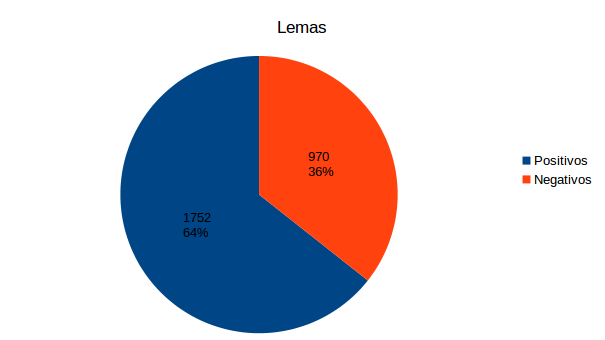
\includegraphics[width=0.8\textwidth]{./fig/Lemas.png}
  \caption{Cantidad de lemas}
  \label{fig:lemas}
\end{figure} 
Se grafica la cantidad de lemas obtenidos luego del procesamiento de datos[\ref{fig:lemas}].

\subsubsection{Comentarios}
\begin{figure}[!h]
  \centering
    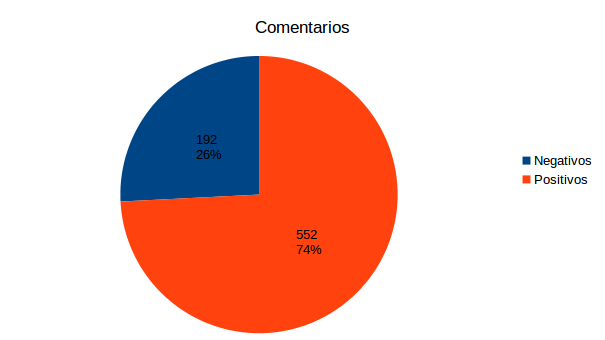
\includegraphics[width=0.8\textwidth]{./fig/Comentarios.png}
  \caption{Cantidad de comentarios}
  \label{fig:com}
\end{figure} 
En este caso, se contabilizan la cantidad de comentarios positivos y negativos[\ref{fig:com}].

\subsubsection{Gráficas}


\begin{figure}[!h]
  \centering
    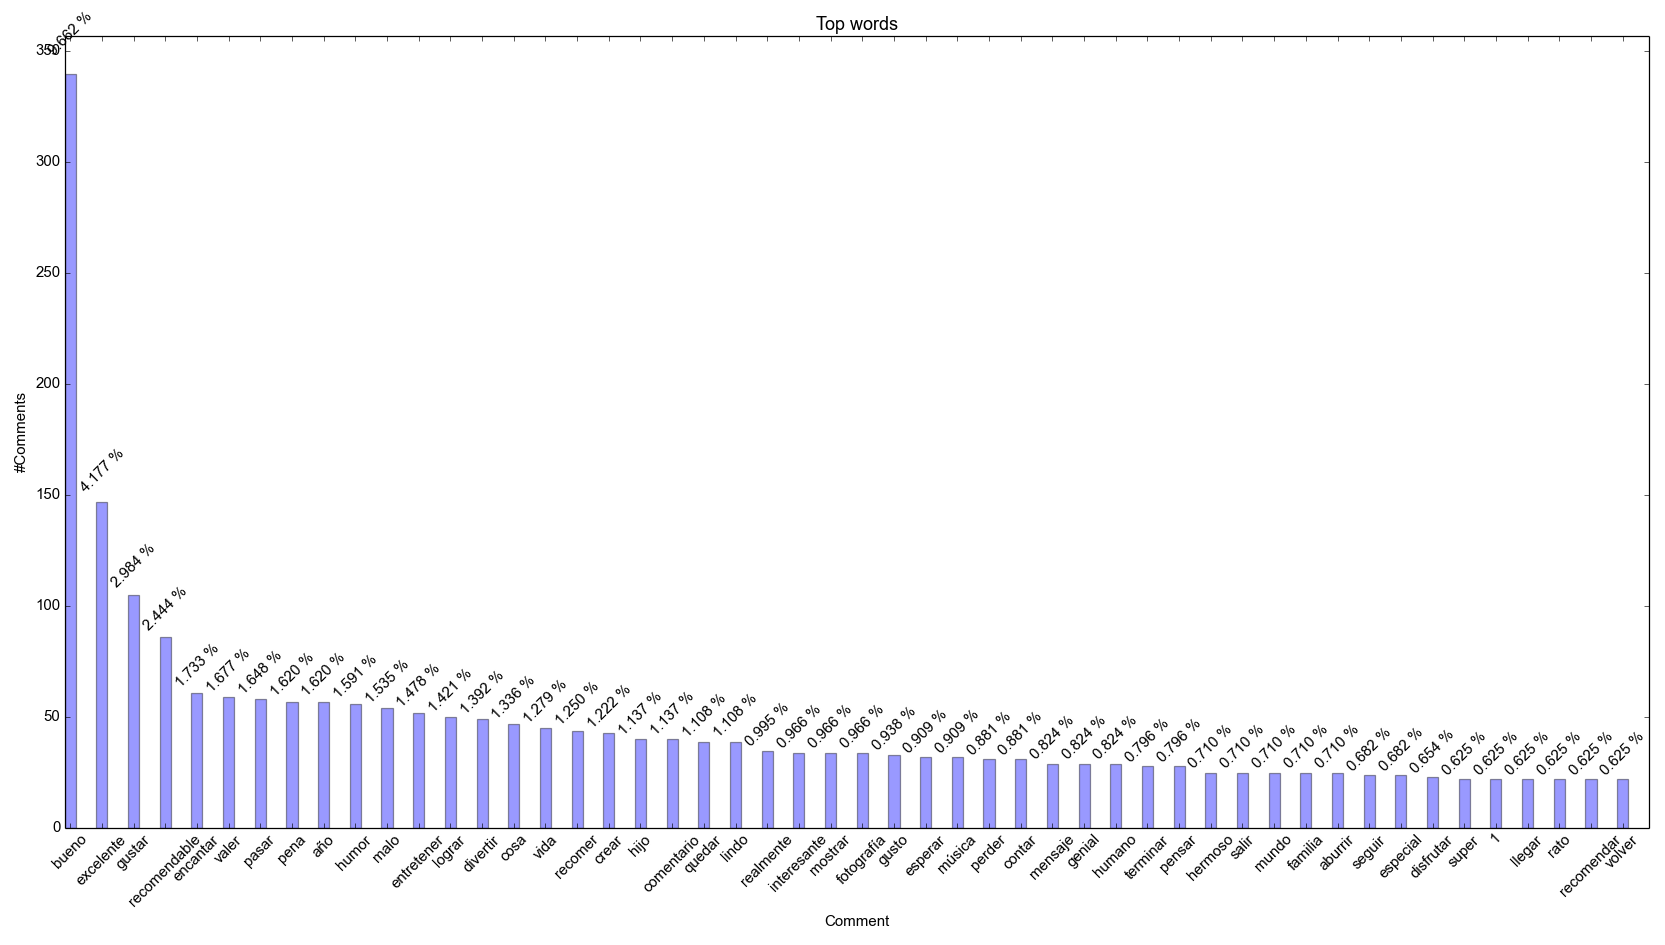
\includegraphics[width=0.8\textwidth]{./fig/AllWords.png}
  \caption{Todas las palabras}
  \label{fig:todas}
\end{figure} 
La gráfica[\ref{fig:todas}] muestra las palabras más encontradas en los comentarios punteados de manera positiva como negativa. Se aprecia en la misma una mayor cantidad de palabras de semántica positiva con respecto a las de semántica negativa.


\begin{figure}[!h]
  \centering
    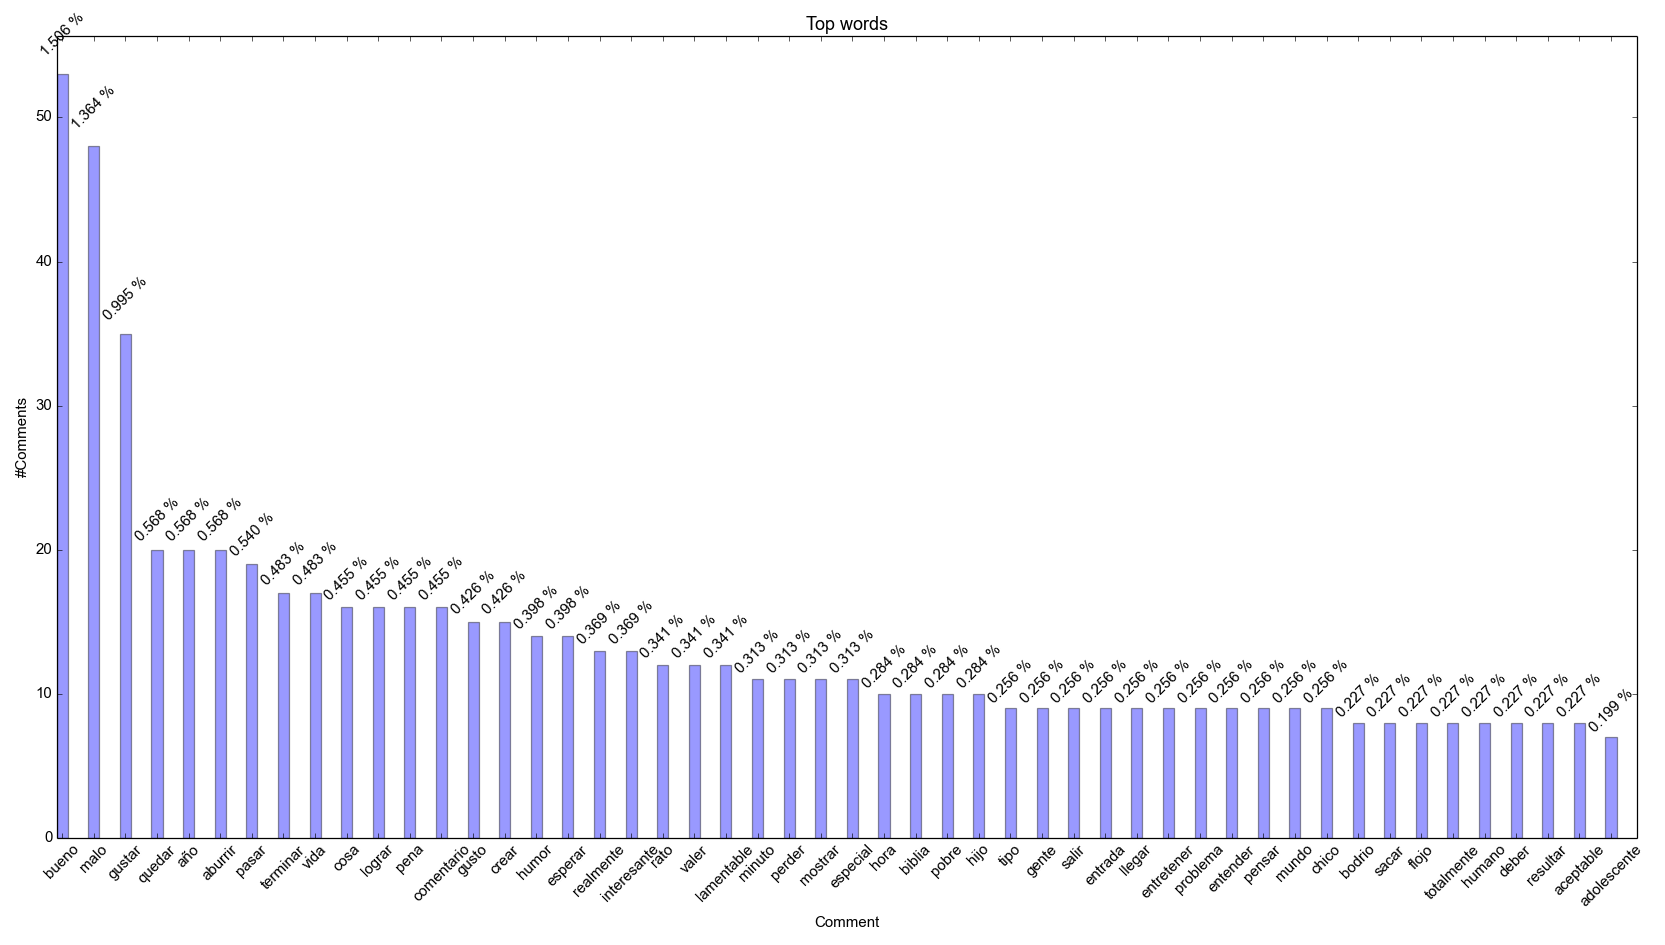
\includegraphics[width=0.8\textwidth]{./fig/NegativeWords.png}
  \caption{Todas las palabras negativas}
  \label{fig:allneg}
\end{figure} 
La gráfica[\ref{fig:allneg}] muestra las palabras más encontradas en los comentarios de puntuación negativa. El bajo porcentaje obtenido de frecuencia de las palabras, se cree que es debido al ruido que poseen los datos, que lleva a que se obtengan resultados no del todo fiables. Se observa la presencia de las palabras “ver”, “película'”, “haber”,”pelicula”,”bueno” ,”gustar” entre las primeras con mayor frecuencia, como también sucede en el caso de la gráfica de todas las palabras.


\begin{figure}[!h]
  \centering
    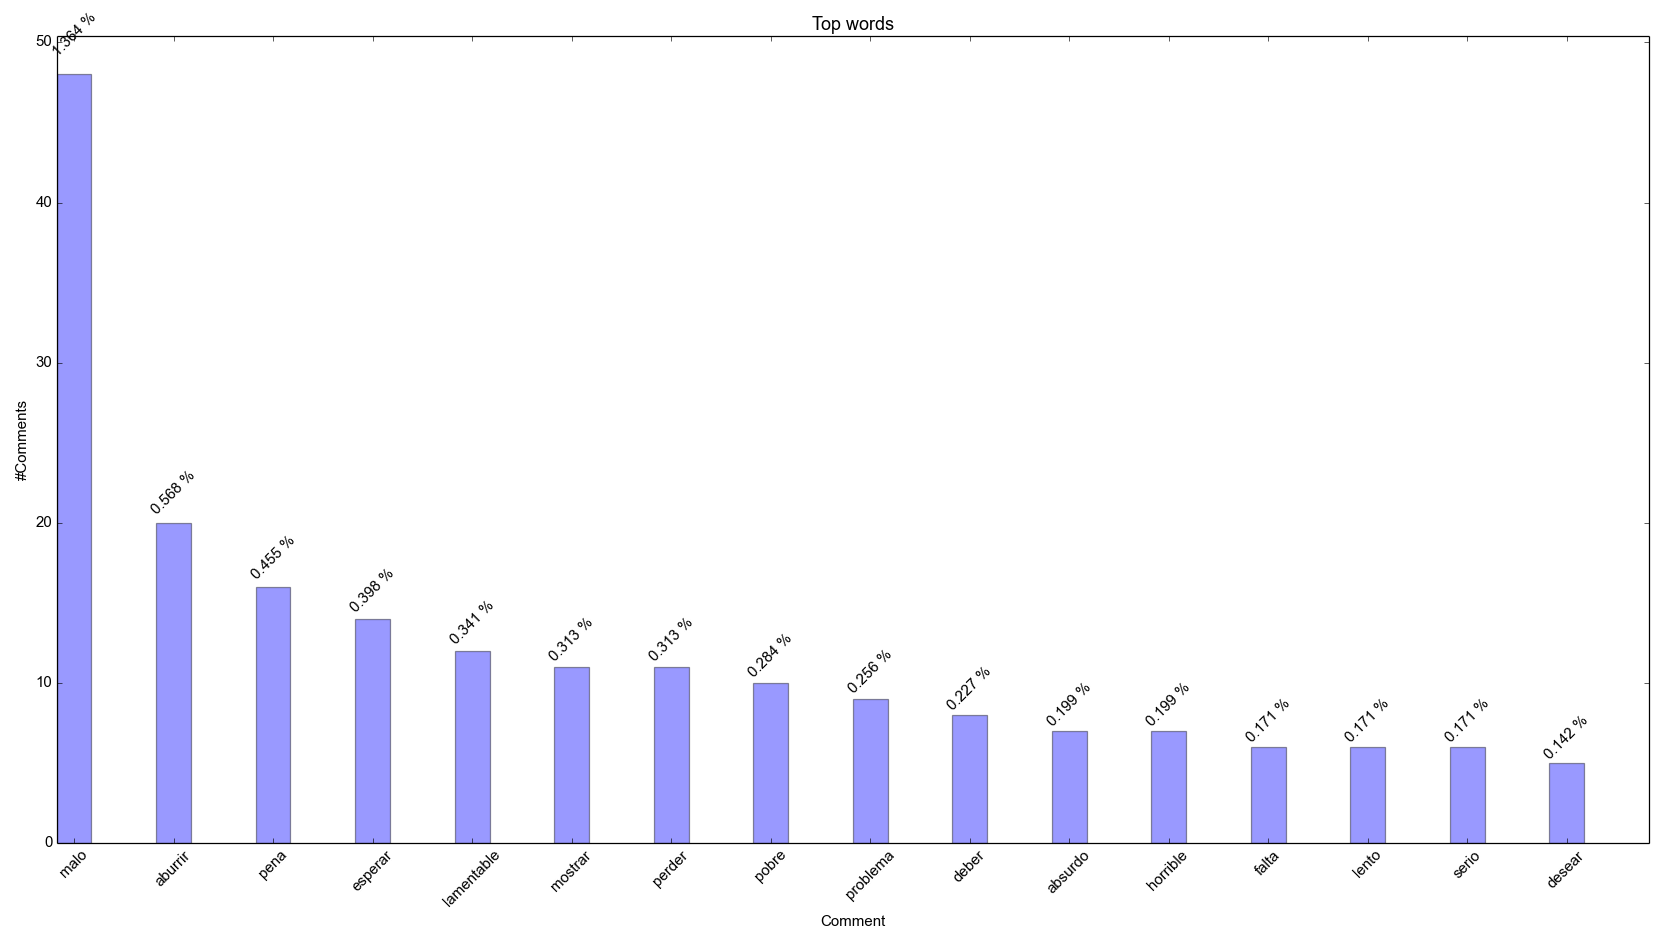
\includegraphics[width=0.8\textwidth]{./fig/NegativeSubjetive.png}
  \caption{Intersección palabras negativas}
  \label{fig:negsub}
\end{figure} 

La gráfica[\ref{fig:negsub}] también se observa los bajos valores de los porcentajes de las palabras encontradas, se cree que esto es debido al ruido que poseen los datos como se explico en la gráfica anterior. En la gráfica se observa una diferencia notoria del termino “malo” con respecto a los otros términos en su frecuencia.


\begin{figure}[!h]
  \centering
    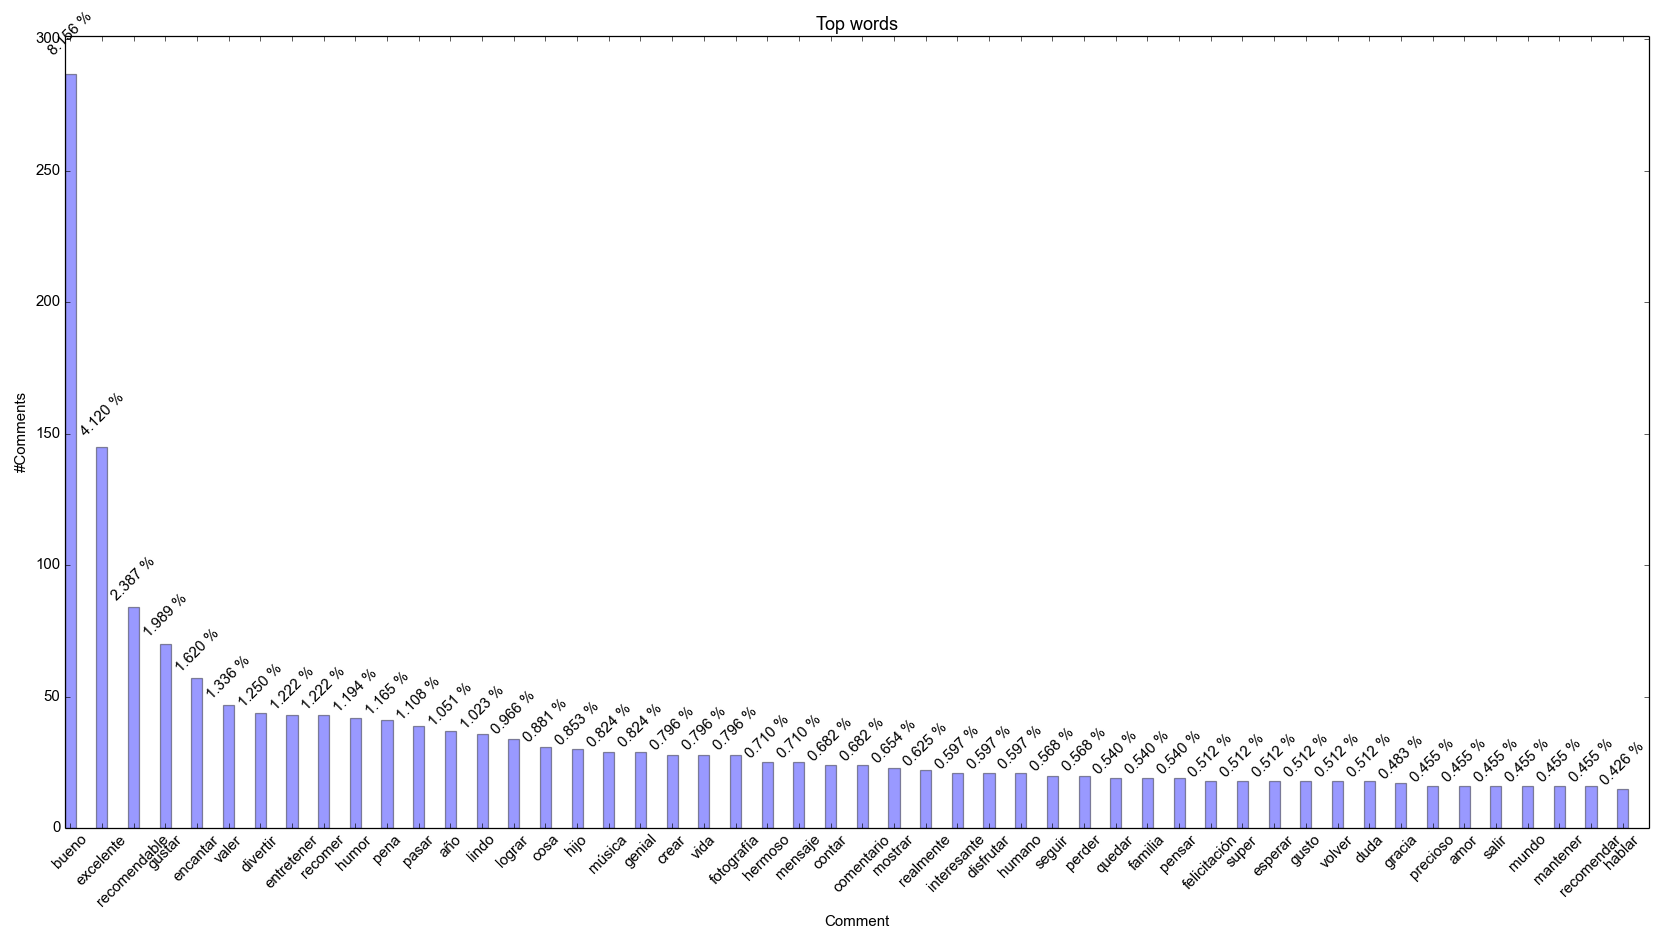
\includegraphics[width=0.8\textwidth]{./fig/PositiveWords.png}
  \caption{Todas las palabras positivas}
  \label{fig:pos}
\end{figure} 

La gráfica[\ref{fig:pos}] muestra las palabras más encontradas en los comentarios de puntuación positiva. El bajo porcentaje obtenido de frecuencia de las palabras, se cree que es debido al ruido que poseen los datos, que lleva a que se obtenegan resultados no del todo fiables. Se observa la presencia de las palabras “ver”, “película'”, “haber”,”pelicula”,”bueno” ,”gustar” entre las primeras con mayor frecuencia, como también sucede en el caso de la gráfica de todas las palabras y la gráfica correspondiente al Top de las palabras negativas. Se observa una mayor frecuencia de los términos “bueno” y “película” con respecto a los otros.


\begin{figure}[!h]
  \centering
    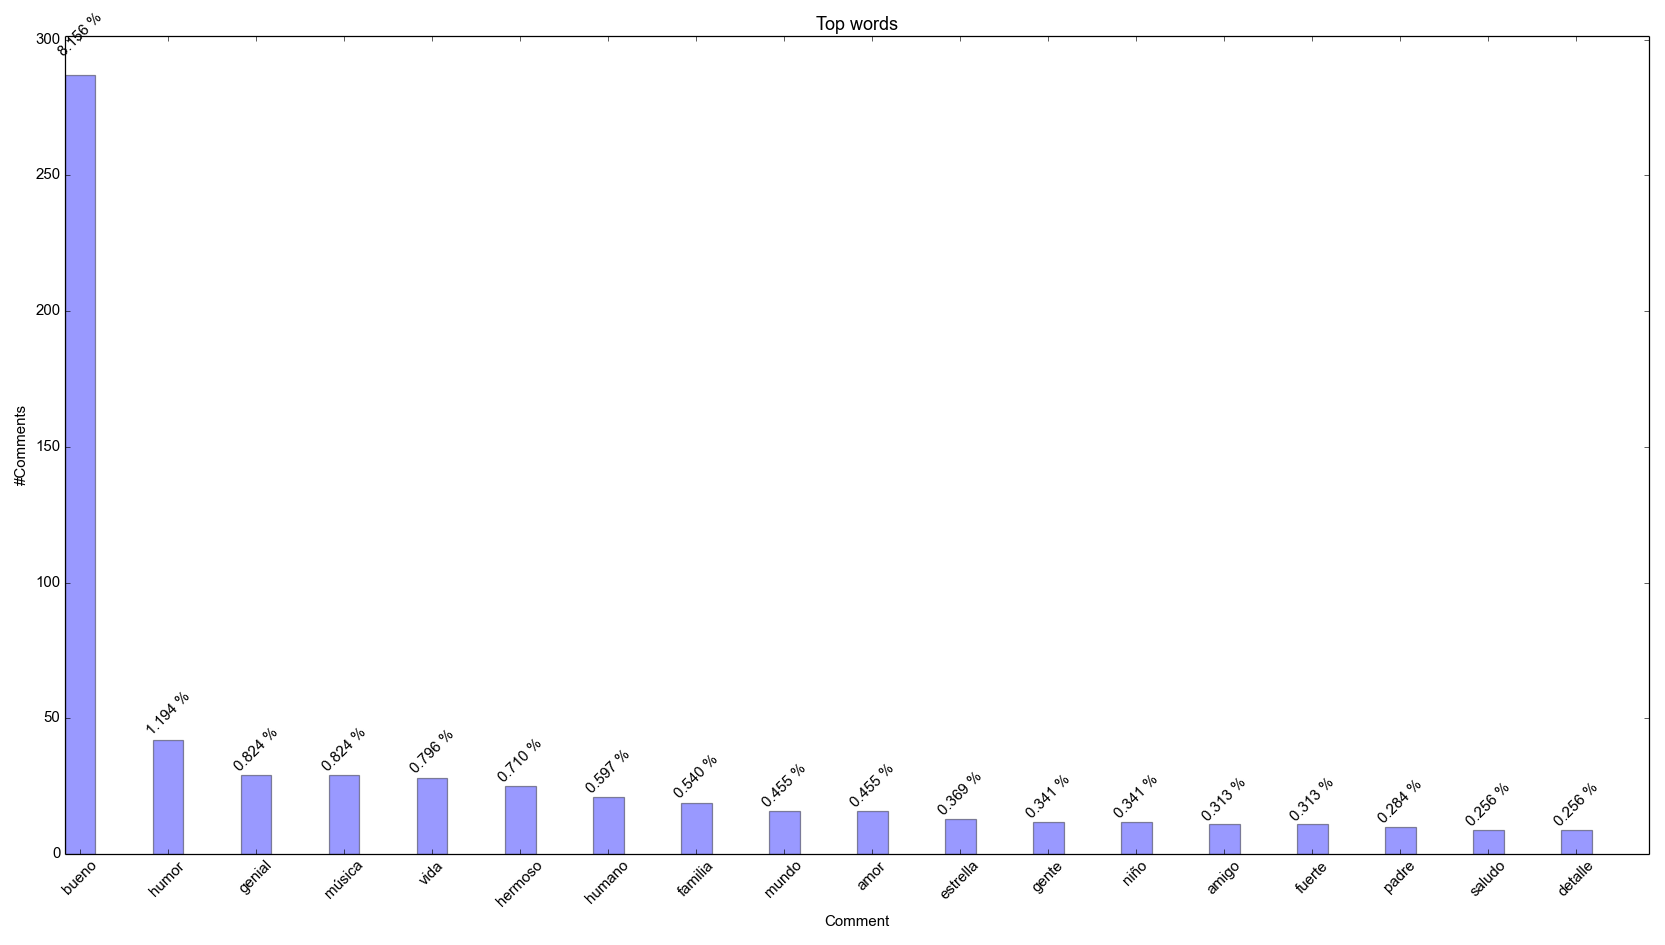
\includegraphics[width=0.8\textwidth]{./fig/PositiveSubjetiveWords.png}
  \caption{Intersección palabras positivas}
  \label{fig:possub}
\end{figure} 


La gráfica[\ref{fig:possub}] también se observa los bajos valores de los porcentajes de las palabras encontradas, se cree que esto es debido al ruido que poseen los datos como se explico anteriormente. En la gráfica se observa una diferencia notoria de los terminos “bueno” y “película” con respecto a los otros terminos en su frecuencia. Estos terminos también son los términos de mayor frecuencia en la gráfica Top palabras positivas.

\section{Conclusiones}\label{conclusions}
Se detallan algunas puntos a tener en cuenta luego de finalizada la presente tarea, se realizan algunos comentarios sobre la implementación.

\subsection{Implementación}
Lenguaje de programación alto nivel, presenta gran diversidad de librerías internas como externas que facilitan la tarea en gran parte. Su alto nivel permite no definir tipos específicos y de esta forma se trabaja de manera más fluida, aunque esto pueda llegar a confusiones si no se declaran correctamente las variables con un nombre adecuado.
Escaso tiempo de implementación, dada la versatilidad, el tiempo de implementación se reduce considerablemente considerando con otros lenguajes de programación.
Al ser lenguaje interpretado, es sencillo de utilizarlo para realizar tareas de menor porte que requieran una cantidad de datos moderado. Se desconoce funcionamiento con gran cantidad de comentarios(potencialmente superior a el caso propuesto).
Codificación legible, si se utilizan estándares como el propuesto en la implementación(PEP8), brinda a terceros la posibilidad de tener un código legible y simple a la lectura.
Portabilidad con sistemas operativos no es 100\% satisfactorio, para desarrollar existieron problemas específicamente de codificación de las palabras, en entornos UNIX no existe dicho problema, mientras que en sistemas Windows existieron los problemas mencionados, además de todo el proceso de instalación del lenguaje(tedioso en Windows) así como también las herramientas(Freeling).
Salvo detalles menores es un lenguaje adecuado para utilizarlo para el procesamiento de datos a pequeña y mediana escala.
Al brindar características de un paradigma funcional(map, zip, etc), brinda simplicidad y 'ahorro' en cantidad de líneas utilizadas en total.
La unificación derivada de la programación lógica, combinada con paradigma funcional hace un lenguaje poderoso con lo que refiere manipulación de datos en general, una característica deseable también como  ser la posibilidad de generar APIs con swig y combinar la eficiencia de c++ en la ejecución de algoritmos que requieran uso excesivo del recurso CPU. 





%\bibliographystyle{abbrv}
%\bibliography{simple}

\end{document}
